% Taken from: https://mikedewar.wordpress.com/2009/02/25/latex-beamer-python-beauty/
\documentclass[12pt,english,pdf,xcolor=dvipsnames,aspectratio=169,handout]{beamer}\usepackage[]{graphicx}\usepackage[]{xcolor}
% maxwidth is the original width if it is less than linewidth
% otherwise use linewidth (to make sure the graphics do not exceed the margin)
\makeatletter
\def\maxwidth{ %
  \ifdim\Gin@nat@width>\linewidth
    \linewidth
  \else
    \Gin@nat@width
  \fi
}
\makeatother

\definecolor{fgcolor}{rgb}{0.345, 0.345, 0.345}
\newcommand{\hlnum}[1]{\textcolor[rgb]{0.686,0.059,0.569}{#1}}%
\newcommand{\hlstr}[1]{\textcolor[rgb]{0.192,0.494,0.8}{#1}}%
\newcommand{\hlcom}[1]{\textcolor[rgb]{0.678,0.584,0.686}{\textit{#1}}}%
\newcommand{\hlopt}[1]{\textcolor[rgb]{0,0,0}{#1}}%
\newcommand{\hlstd}[1]{\textcolor[rgb]{0.345,0.345,0.345}{#1}}%
\newcommand{\hlkwa}[1]{\textcolor[rgb]{0.161,0.373,0.58}{\textbf{#1}}}%
\newcommand{\hlkwb}[1]{\textcolor[rgb]{0.69,0.353,0.396}{#1}}%
\newcommand{\hlkwc}[1]{\textcolor[rgb]{0.333,0.667,0.333}{#1}}%
\newcommand{\hlkwd}[1]{\textcolor[rgb]{0.737,0.353,0.396}{\textbf{#1}}}%
\let\hlipl\hlkwb

\usepackage{framed}
\makeatletter
\newenvironment{kframe}{%
 \def\at@end@of@kframe{}%
 \ifinner\ifhmode%
  \def\at@end@of@kframe{\end{minipage}}%
  \begin{minipage}{\columnwidth}%
 \fi\fi%
 \def\FrameCommand##1{\hskip\@totalleftmargin \hskip-\fboxsep
 \colorbox{shadecolor}{##1}\hskip-\fboxsep
     % There is no \\@totalrightmargin, so:
     \hskip-\linewidth \hskip-\@totalleftmargin \hskip\columnwidth}%
 \MakeFramed {\advance\hsize-\width
   \@totalleftmargin\z@ \linewidth\hsize
   \@setminipage}}%
 {\par\unskip\endMakeFramed%
 \at@end@of@kframe}
\makeatother

\definecolor{shadecolor}{rgb}{.97, .97, .97}
\definecolor{messagecolor}{rgb}{0, 0, 0}
\definecolor{warningcolor}{rgb}{1, 0, 1}
\definecolor{errorcolor}{rgb}{1, 0, 0}
\newenvironment{knitrout}{}{} % an empty environment to be redefined in TeX

\usepackage{alltt}
\usepackage{etex}
\usetheme{default}
\beamertemplatenavigationsymbolsempty
\definecolor{fore}{RGB}{43,41,46}
\definecolor{back}{RGB}{255,255,255}
\definecolor{title}{RGB}{198,24,38}
\setbeamercolor{titlelike}{fg=title}
\setbeamercolor{normal text}{fg=fore,bg=back}
\usepackage{mathpazo}
\usepackage{amsmath}
\usepackage{multirow}
\renewcommand{\familydefault}{\rmdefault}
\usepackage[T1]{fontenc}
\usepackage{inputenc}
\usepackage{parskip}
\setcounter{secnumdepth}{3}
\setcounter{tocdepth}{3}
\usepackage{hyperref}
\hypersetup{pdfauthor={Constantin Manuel Bosancianu},
pdftitle={Advanced Topics in Applied Regression},
pdfsubject={Day 3: Interactions & fixed-effects},
pdfkeywords={Budapest, ECPR, 2017, day 3, SSMT}}
\usepackage{babel}
\usepackage{graphicx}
\usepackage{subfigure}
\usepackage{palatino}
% Defines a checkmark
\def\checkmark{\tikz\fill[scale=0.4,color=title](0,.35) -- (.25,0) -- (1,.7) -- (.25,.15) -- cycle;}
\setbeamertemplate{itemize items}{\checkmark}
% For table captions in Beamer
\usepackage[labelformat=empty]{caption}
\captionsetup[figure]{labelfont={color=fore}}
\captionsetup[table]{labelfont={color=fore}}
\usepackage{tikz, tikz-cd, animate}
\usetikzlibrary{shapes,backgrounds,trees}
\usetikzlibrary{decorations.pathreplacing}
\usepackage{pgfplots}
\pgfplotsset{compat=1.10}
\usepgfplotslibrary{fillbetween}
\usepackage{pgfplotstable}
\usepackage{wrapfig}
\usepackage{booktabs}
\usepackage{dcolumn}
\usepackage[sectionbib]{apacite}
\renewcommand{\bibliographytypesize}{\footnotesize}
% Set the design of the footer
\makeatletter
\setbeamercolor{author in head/foot}{fg=white, bg=title}
\setbeamercolor{date in head/foot}{fg=white, bg=title}
\setbeamercolor{institute in head/foot}{fg=white, bg=title}
\setbeamertemplate{footline}
{
  \leavevmode%
  \hbox{%
  \begin{beamercolorbox}[wd=.3333333\paperwidth,ht=2.25ex,dp=1ex,center]{author in head/foot}%
    \usebeamerfont{author in head/foot}\insertauthor
  \end{beamercolorbox}%
    \begin{beamercolorbox}[wd=.3333333\paperwidth,ht=2.25ex,dp=1ex,center]{institute in head/foot}%
    \usebeamerfont{institute in head/foot}Central European University, Budapest
  \end{beamercolorbox}%
  \begin{beamercolorbox}[wd=.3333333\paperwidth,ht=2.25ex,dp=1ex,right]{date in head/foot}%
    \usebeamerfont{date in head/foot}\insertshortdate{}\hspace*{2em}
    \insertframenumber{} / \inserttotalframenumber\hspace*{2ex}
  \end{beamercolorbox}}%
  \vskip0pt%
}
\makeatother
\title{Advanced Topics in Applied Regression}
\subtitle{Day 3: Interactions \& fixed-effects}
\author{Constantin Manuel Bosancianu}
\institute{Doctoral School of Political Science \\ Central European University, Budapest\\\href{mailto:bosancianu@icloud.com}{bosancianu@icloud.com}}
\date{August 2, 2017}
\IfFileExists{upquote.sty}{\usepackage{upquote}}{}
\begin{document}
\maketitle



% PREAMBLE %
\section{Preamble}

\begin{frame}{Why interactions?}

They allow for a much richer set of hypotheses to be put forward and tested.\bigskip

In my own area of focus (political institutions, economic phenomena, and voter attitudes/behavior), such hypotheses involving moderation are very common.\bigskip

One prominent example: income inequality's effect on voter turnout at different levels of a person's income \cite{solt2008}.\bigskip

Despite their importance, misunderstandings still persist about how to interpret coefficients/effects in such models.

\end{frame}






\section{Basic setup}

\begin{frame}
\begin{center}
    \Huge Basic setup
\end{center}
\end{frame}

\begin{frame}{Why specify interactions}

So far, we've worked with simple models. Think of the example from Monday, with Boston neighborhood average house prices. Here, I complicated it a bit by also adding a dummy for whether the neighborhood is on the Charles river or not:

\begin{equation}
Prices = a + b_1Rooms + b_2River + e
\end{equation}

Here, the effect of $River$ is assumed to be constant, $b_2$, no matter the level of the other variable in the model.\bigskip

This is not always the case: effect of SES and union membership on political participation, where $b_{union}$ likely varies.

\end{frame}



\begin{frame}{What if the effect isn't constant?}

The riverfront is a desirable real-estate location. Houses with more rooms are certainly more expensive everywhere in Boston, but it's likely that the price difference between $n+1$ and $n$ rooms is higher on the riverfront than elsewhere.\bigskip

In modelling terms, we might say that the effect of $Rooms$ on $Price$ is different based on the value of the $River$ dummy.

\end{frame}


\begin{frame}{From words to equation (I)}

\begin{align}
Prices =& a_1 + b_1Rooms + b_2River + e \nonumber\\
b_1 =& a_2 + b_3River \nonumber\\
a_1 =& a_3 + b_4River \nonumber
\end{align}

The second equation gives us how the effect of $Rooms$ ($b_1$) varies depending on $River$.\bigskip

The third equation makes sure that the intercept varies as well (which usually happens if the slope varies).

\end{frame}


\begin{frame}{From words to equation (II)}

{\footnotesize
\begin{align}
Prices =& a_3 + b_4River + (a_2 + b_3River)*Rooms + b_2River + e \nonumber\\
  =& a_3 + (b_4+b_2)*River + a_2Rooms + b_3River*Rooms + e \nonumber \\
  =& a_3 + (b_4+b_2)*River + (a_2+b_3River)*Rooms + e
\end{align}
}%

The third row shows most clearly how the effect of $Rooms$, $a_2+b_3River$, now varies depending on the precise value of the $River$ indicator.\bigskip

This depends, of course, on the $b_3$ being statistically significant. If not, then the effect of $Rooms$ is always $a_2$.

\end{frame}


\begin{frame}{Basic interaction model}

\begin{equation}
  \footnotesize
  Prices = a_3 + (b_4+b_2)*River + (a_2+b_3River)*Rooms + e
\end{equation}\bigskip

 If we designate $a_3$ as $\gamma_1$, $b_4+b_2$ as $\gamma_2$, $a_2$ as $\gamma_3$, and $b_3$ as $\gamma_4$, then we get a general form of the interaction:\bigskip

\begin{equation}
  \footnotesize
  Prices = \gamma_1 + \gamma_2River + \gamma_3Rooms + \gamma_4River*Rooms + e
\end{equation}
 
\end{frame}



\begin{frame}{Interaction model (cont.)}

When $River=0$,

\begin{align}
  Prices =& \gamma_1 + \gamma_20 + \gamma_3Rooms + \gamma_4Rooms*0 + e \nonumber\\
         =& \gamma_1 + \gamma_3Rooms + e
\end{align}

When $River=1$,

\begin{align}
  Prices =& \gamma_1 + \gamma_21 + \gamma_3Rooms + \gamma_4Rooms*1 + e \nonumber\\
         =& \gamma_1 + \gamma_2 + Rooms(\gamma_3 + \gamma_4) + e
\end{align}

The effect of $Rooms$ varies depending on the value of $River$.

\end{frame}




\begin{frame}{Symmetry in interpretation}

When $Rooms=0$, then

\begin{align}
  Prices =& \gamma_1 + \gamma_2River + \gamma_3*0 + \gamma_4River*0 + e \nonumber\\
         =& \gamma_1 + \gamma_2River + e \nonumber
\end{align}

When $Rooms=1$,

\begin{align}
  Prices =& \gamma_1 + \gamma_2River + \gamma_3*1 + \gamma_4River*1 + e \nonumber\\
         =& \gamma_1 + \gamma_3 + River(\gamma_2 + \gamma_4) + e \nonumber
\end{align}

The effect of $River$ varies depending on the level of $Rooms$.

\end{frame}





\section{Interpreting coefficients}


\begin{frame}
\begin{center}
    \Huge Interpretation
\end{center}
\end{frame}


\begin{frame}{Wages in 1976}
We have information on 526 US workers:

\begin{itemize}
\item \texttt{wage}: wage in USD per hour;
\item \texttt{educ}: years of education;
\item \texttt{gender}: male or female (with 1=female);
\item \texttt{exper}: labor force experience (yrs. in labor market);
\item \texttt{tenure}: yrs. with current employer.
\end{itemize}

The goal is to predict wages.\footnote{In fact, we'll be predicting $log(wage)$, as wages tend to be right skewed, which causes problems with the normality of errors.}

\end{frame}


\begin{frame}[fragile]{Interpreting coefficients}

\begin{table}
\caption{Specification with interaction: Female * Tenure}
\begin{center}
\begin{scriptsize}
\begin{tabular}{l D{.}{.}{3.6}}
\toprule
 & \multicolumn{1}{c}{DV: Log hourly wage (USD)} \\
\midrule
(Intercept)     & 1.762^{***}  \\
                & (0.025)      \\
Female          & -0.311^{***} \\
                & (0.037)      \\
Yrs. education  & 0.089^{***}  \\
                & (0.007)      \\
Yrs. experience & 0.005^{**}   \\
                & (0.002)      \\
Yrs. tenure     & 0.021^{***}  \\
                & (0.003)      \\
Female * Tenure & -0.013^{*}   \\
                & (0.006)      \\
\midrule
R$^2$           & 0.399        \\
Adj. R$^2$      & 0.393        \\
Num. obs.       & 526          \\
\bottomrule
\multicolumn{2}{l}{\tiny{$^{***}p<0.001$; $^{**}p<0.01$; $^{*}p<0.05$. Continuous variables were demeaned.}}
\end{tabular}
\end{scriptsize}
\label{table:coefficients}
\end{center}
\end{table}

\end{frame}



\begin{frame}{Interpreting coefficients (cont.)}
How do you interpret $\beta_{female}=-0.311$?\bigskip

\textcolor{title}{Important}: after demeaning, the ``0'' for variable $X$ refers to the mean of $X$, $\overline{X}$.\bigskip

How do you interpret $\beta_{tenure}=NA$?\bigskip

How do you interpret $\beta_{female*tenure}=NA$? How is the effect of $tenure$ different for men, compared to women?

\end{frame}



\begin{frame}[fragile]{Graphical depiction}
  
\begin{figure}[!ht]
\centering
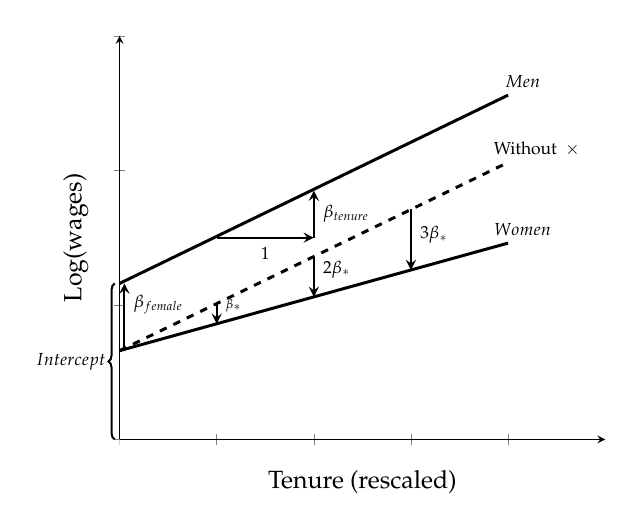
\begin{tikzpicture}[scale=0.9]
\begin{axis}[
	xlabel=Tenure (rescaled), % label x axis
	ylabel=Log(wages), % label y axis
	axis lines=left, %set the position of the axes
	xmin=0, xmax=10, % set the min and max values of the x-axis
	ymin=1.7, ymax=2.0, % set the min and max values of the y-axis
	xticklabels={,,}, % Hide tick labels
	yticklabels={,,},
	clip=false
]

\draw [very thick] (0,116)--(80,256);
\draw [very thick, dashed] (0,66)--(80,206);
\draw [very thick] (0,66)--(80,146);
\draw [thick,->,>=stealth] (1,66)--(1,116) node [midway,right, yshift=5pt] {\scriptsize{$\beta_{female}$}};
\draw [thick,->,>=stealth] (20,150)--(40,150) node [midway,below] {\scriptsize{$1$}};
\draw [thick,->,>=stealth] (40,150)--(40,185) node [midway,right] {\scriptsize{$\beta_{tenure}$}};
\node [fill=none] at (83, 156) {\scriptsize{$Women$}};
\node [fill=none] at (83, 266) {\scriptsize{$Men$}};
\node [fill=none, text width=1.5cm] at (88, 216) {\scriptsize{Without $\times$}};
\draw[decorate,decoration={brace}, thick] (-1,0) -- node[left] {\scriptsize{$Intercept$}} (-1,116);
% Add the arrows for the interaction
\draw [thick,->,>=stealth] (20,101)--(20,86) node [midway,right, yshift=3pt] {\tiny{$\beta_{*}$}};
\draw [thick,->,>=stealth] (40,136)--(40,106) node [midway,right, yshift=3pt] {\scriptsize{$2\beta_{*}$}};
\draw [thick,->,>=stealth] (60,171)--(60,126) node [midway,right, yshift=2pt] {\scriptsize{$3\beta_{*}$}};
\end{axis}
\end{tikzpicture}
\caption{Example with wages (graph adapted from \citeNP{brambor2005}). $\beta_{*}$ means $\beta_{female*tenure}$.}
\end{figure}

\end{frame}




\begin{frame}[fragile]{Difference between \textit{coefficients} and \textit{effects}}

For linear models without interactions, $coefficient=effect$. A $\beta_X=2$ means the \textit{effect} of 1-unit increase in $X$ on $Y$ is 2.\bigskip

For linear models with (significant) interactions, $coefficient \neq effect$. Rather, the effect of an interacted variable is a function of 2 coefficients.\bigskip

{\footnotesize
\begin{align}
Wage =& 1.762 - 0.311*Fem. + 0.021*Tnr. - 0.013*Fem.*Tnr. + \dots \nonumber \\
     =& 1.762 + 0.021*Tnr. + \underbrace{(-0.311-0.013*Tnr.)}_{\text{effect}}*Fem. + \dots \nonumber
\end{align}
}%

\end{frame}



\begin{frame}{2nd example: differences in salaries}


\begin{table}
\caption{Experience measured in years, management is dichotomous indicator (1=manager)}
\begin{center}
\begin{footnotesize}
\begin{tabular}{l D{.}{.}{5.5}}
\toprule
 & \multicolumn{1}{c}{DV: Salary in company} \\
\midrule
(Intercept)     & 14180.85^{***} \\
                & (333.93)       \\
Experience      & 452.66^{***}   \\
                & (60.18)        \\
Management      & 7172.32^{***}  \\
                & (506.82)       \\
Exper.*Managem. & 222.74^{*}     \\
                & (104.09)       \\
\midrule
R$^2$           & 0.88           \\
Adj. R$^2$      & 0.87           \\
Num. obs.       & 46             \\
\bottomrule
\multicolumn{2}{l}{\tiny{$^{***}p<0.001$; $^{**}p<0.01$; $^{*}p<0.05$. Experience has been centered by subtracting 7.5 from each value.}}
\end{tabular}
\end{footnotesize}
\label{table:coefficients}
\end{center}
\end{table}


\end{frame}



\begin{frame}{3rd example: Boston house prices}


\begin{table}
\caption{Predicting house price in neighborhood}
\begin{center}
\begin{footnotesize}
\begin{tabular}{l D{.}{.}{3.6} D{.}{.}{3.6}}
\toprule
 & \multicolumn{1}{c}{Model 1} & \multicolumn{1}{c}{Model 2} \\
\midrule
(Intercept)        & 22.251^{***} & 22.250^{***} \\
                   & (0.302)      & (0.301)      \\
Average num. rooms & 9.024^{***}  & 8.967^{***}  \\
                   & (0.440)      & (0.416)      \\
Charles river      & 4.194^{***}  & 4.083^{***}  \\
                   & (1.186)      & (1.151)      \\
Charles*Rooms      & -0.536       &              \\
                   & (1.355)      &              \\
\midrule
R$^2$              & 0.496        & 0.496        \\
Adj. R$^2$         & 0.493        & 0.494        \\
Num. obs.          & 506          & 506          \\
\bottomrule
\multicolumn{3}{l}{\tiny{$^{***}p<0.001$; $^{**}p<0.01$; $^{*}p<0.05$. Number of rooms has been demeaned.}}
\end{tabular}
\end{footnotesize}
\label{table:coefficients}
\end{center}
\end{table}


\end{frame}




\begin{frame}{Interactions -- other measurement scales}

The interpretations carry over perfectly, e.g. when both are continuous (we will practice more during the lab).\bigskip

\begin{equation}
Y = a + b_1X_1 + b_2X_2 + b_3(X_1*X_2) + e
\end{equation}\bigskip

$b_2$ is the effect of $X_2$ on $Y$ when $X_1$ is 0.\bigskip

The converse interpretation, for $b_1$, is also identical.

\end{frame}




\section{Collinearity}


\begin{frame}
\begin{center}
    \Huge Collinearity
\end{center}
\end{frame}


\begin{frame}[fragile]{High correlations in interactions}

\begin{knitrout}\scriptsize
\definecolor{shadecolor}{rgb}{0.969, 0.969, 0.969}\color{fgcolor}\begin{kframe}
\begin{alltt}
\hlstd{out} \hlkwb{<-} \hlkwd{mvrnorm}\hlstd{(}\hlnum{300}\hlstd{,} \hlcom{# number of observations}
               \hlkwc{mu} \hlstd{=} \hlkwd{c}\hlstd{(}\hlnum{5}\hlstd{,} \hlnum{5}\hlstd{),} \hlcom{# means of the variables}
               \hlcom{# correlation matrix}
               \hlkwc{Sigma} \hlstd{=} \hlkwd{matrix}\hlstd{(}\hlkwd{c}\hlstd{(}\hlnum{1}\hlstd{,} \hlnum{0.35}\hlstd{,} \hlnum{0.35}\hlstd{,} \hlnum{1}\hlstd{),} \hlkwc{ncol} \hlstd{=} \hlnum{2}\hlstd{),}
               \hlkwc{empirical} \hlstd{=} \hlnum{TRUE}\hlstd{)}
\hlkwd{colnames}\hlstd{(out)} \hlkwb{<-} \hlkwd{c}\hlstd{(}\hlstr{"x1"}\hlstd{,} \hlstr{"x2"}\hlstd{)}
\hlstd{out} \hlkwb{<-} \hlkwd{as.data.frame}\hlstd{(out)}
\hlkwd{cor}\hlstd{(out}\hlopt{$}\hlstd{x1, out}\hlopt{$}\hlstd{x2)} \hlcom{# So, that's the correlation}
\end{alltt}
\begin{verbatim}
[1] 0.35
\end{verbatim}
\begin{alltt}
\hlstd{out}\hlopt{$}\hlstd{inter} \hlkwb{<-} \hlstd{out}\hlopt{$}\hlstd{x1} \hlopt{*} \hlstd{out}\hlopt{$}\hlstd{x2} \hlcom{# Construct the interaction term}
\hlkwd{cor}\hlstd{(out}\hlopt{$}\hlstd{x1, out}\hlopt{$}\hlstd{inter)} \hlcom{# Correlation}
\end{alltt}
\begin{verbatim}
[1] 0.8133725
\end{verbatim}
\begin{alltt}
\hlkwd{cor}\hlstd{(out}\hlopt{$}\hlstd{x2, out}\hlopt{$}\hlstd{inter)} \hlcom{# Correlation}
\end{alltt}
\begin{verbatim}
[1] 0.818435
\end{verbatim}
\end{kframe}
\end{knitrout}

In these situations, the VIF becomes very large, making the sampling variance for coefficients large as well.

\end{frame}




\begin{frame}[fragile]{High correlations -- ``solution''}

Essentially, it's justified that we have large SEs---the software is telling us it doesn't have enough \textit{unique} information to estimate the effect precisely.\bigskip

The ``solution'': center the variable, i.e. subtract the mean/median from all observations on the variable.\bigskip

\begin{equation}
X_i^{*} = X_i - \overline{X}
\end{equation}

\end{frame}




\begin{frame}[fragile]{High correlations -- ``solution''}

\begin{knitrout}\scriptsize
\definecolor{shadecolor}{rgb}{0.969, 0.969, 0.969}\color{fgcolor}\begin{kframe}
\begin{alltt}
\hlstd{out}\hlopt{$}\hlstd{x1mod} \hlkwb{<-} \hlstd{out}\hlopt{$}\hlstd{x1} \hlopt{-} \hlkwd{mean}\hlstd{(out}\hlopt{$}\hlstd{x1)}
\hlstd{out}\hlopt{$}\hlstd{x2mod} \hlkwb{<-} \hlstd{out}\hlopt{$}\hlstd{x2} \hlopt{-} \hlkwd{mean}\hlstd{(out}\hlopt{$}\hlstd{x2)}
\hlkwd{cor}\hlstd{(out}\hlopt{$}\hlstd{x1mod, out}\hlopt{$}\hlstd{x2mod)} \hlcom{# cor(X1,X2) is the same}
\end{alltt}
\begin{verbatim}
[1] 0.35
\end{verbatim}
\begin{alltt}
\hlstd{out}\hlopt{$}\hlstd{intermod} \hlkwb{<-} \hlstd{out}\hlopt{$}\hlstd{x1mod} \hlopt{*} \hlstd{out}\hlopt{$}\hlstd{x2mod}
\hlkwd{cor}\hlstd{(out}\hlopt{$}\hlstd{x1mod, out}\hlopt{$}\hlstd{intermod)} \hlcom{# Correlation}
\end{alltt}
\begin{verbatim}
[1] -0.05324645
\end{verbatim}
\begin{alltt}
\hlkwd{cor}\hlstd{(out}\hlopt{$}\hlstd{x2mod, out}\hlopt{$}\hlstd{intermod)} \hlcom{# Correlation}
\end{alltt}
\begin{verbatim}
[1] -0.01015134
\end{verbatim}
\end{kframe}
\end{knitrout}

Not so much a solution; more of a \textit{re-specification} of the original model \cite[pp.~93--99]{kam2007}.

Centering will produce different $b$s, $a$ and SEs, simply because these refer to different quantities.\bigskip

\end{frame}




\section{Presenting uncertainty and results}


\begin{frame}
\begin{center}
    \Huge Presentation
\end{center}
\end{frame}


\begin{frame}{Significance testing in interactions}
With interactions, significance tests also take on a different interpretation \cite{braumoeller2004}.\bigskip

\begin{equation}
Y = a + b_1X_1 + b_2X_2 + b_3(X_1*X_2) + e
\end{equation}

The significance test on $b_1$ is only valid for instance when $b_2=0$.\bigskip

At other levels of $b_2$, this significance test might no longer produce a positive result.

\end{frame}


\begin{frame}{Sampling variance}

\begin{equation}
Y = a + b_1X_1 + b_2X_2 + b_3(X_1*X_2) + e
\end{equation}\bigskip

Since it's an interaction, $b_1$ is the coefficient of $X_1$, and $eff_{X_1}$ is the effect of $X_1$ on $Y$. If $b_3$ is significant, $b_1 \neq eff_{X_1}$\bigskip

\begin{equation}
V(eff_{X_1}) = V(b_1) + X_2^2V(b_3) + 2X_2Cov(b_1,b_3)
\label{eq:eq-1}
\end{equation}

This makes it clear that the variance varies depending on $X_2$ as well.

\end{frame}



\begin{frame}{Presenting results}
There is little need to use the formula in Equation \ref{eq:eq-1} to compute things by hand.\footnote{An example that shows you how to do this can be found in today's script.}\bigskip

The best way to do present results from a specification with interactions is by plotting both the effect and its associated uncertainty.\bigskip

An easy way to do this is with the \texttt{effects} package in R (but also check out Thomas Leeper's \texttt{margins} package).

\end{frame}


\begin{frame}{Predicting salaries}

\begin{table}
\caption{Experience measured in years, management is dichotomous indicator (1=manager)}
\begin{center}
\begin{footnotesize}
\begin{tabular}{l D{.}{.}{5.5}}
\toprule
 & \multicolumn{1}{c}{DV: Salary in company} \\
\midrule
(Intercept)     & 14180.85^{***} \\
                & (333.93)       \\
Experience      & 452.66^{***}   \\
                & (60.18)        \\
Management      & 7172.32^{***}  \\
                & (506.82)       \\
Exper.*Managem. & 222.74^{*}     \\
                & (104.09)       \\
\midrule
R$^2$           & 0.88           \\
Adj. R$^2$      & 0.87           \\
Num. obs.       & 46             \\
\bottomrule
\multicolumn{2}{l}{\tiny{$^{***}p<0.001$; $^{**}p<0.01$; $^{*}p<0.05$. Experience has been centered by subtracting 7.5 from each value.}}
\end{tabular}
\end{footnotesize}
\label{table:coefficients}
\end{center}
\end{table}

\end{frame}



\begin{frame}{Predicting salaries -- effect of experience}


\begin{figure}
\centering
\includegraphics{../04-graphs/03-01}
\end{figure}

\end{frame}



\begin{frame}{Predicting salaries -- effect of management}


\begin{figure}
\centering
\includegraphics{../04-graphs/03-02}
\end{figure}

\end{frame}


\begin{frame}{Predicting hourly wage -- 3-way interaction}


\begin{figure}
\centering
\includegraphics[scale=0.75]{../04-graphs/03-03}
\end{figure}

\end{frame}





\section{Fixed effects}

\begin{frame}
\begin{center}
    \Huge Fixed effects
\end{center}
\end{frame}


\begin{frame}{Why fixed effects?}


\begin{table}
\caption{Predicting house price using number of rooms}
\begin{center}
\begin{footnotesize}
\begin{tabular}{l D{.}{.}{3.6}}
\toprule
 & \multicolumn{1}{c}{DV: House price (ave.)} \\
\midrule
(Intercept)        & -42.757^{***} \\
                   & (9.620)       \\
Average num. rooms & 10.139^{***}  \\
                   & (1.568)       \\
\midrule
R$^2$              & 0.471         \\
Adj. R$^2$         & 0.460         \\
Num. obs.          & 49            \\
\bottomrule
\multicolumn{2}{l}{\tiny{$^{***}p<0.001$; $^{**}p<0.01$; $^{*}p<0.05$}}
\end{tabular}
\end{footnotesize}
\label{table:coefficients}
\end{center}
\end{table}


\end{frame}


\begin{frame}{Why fixed effects?}


\begin{figure}
\centering
\includegraphics[scale=0.7]{../04-graphs/03-04}
\end{figure}

\end{frame}


\begin{frame}{Why fixed effects?}

\begin{enumerate}
\item As a solution to the issue of heteroskedasticity, when the problem is caused by different trends in each of the groups.
\item As a solution to the issue of omitted variable bias, on the road to a better causal estimate of the effect of $X$ on $Y$.
\end{enumerate}\bigskip

These two issues are related, inasmuch as the trends in the groups are caused by variables which our model specification does not include.

\end{frame}


\begin{frame}{Classic example}

We have 172 children assessed with a test at 3 points in time.\bigskip

The goal is to understand what predicts their test scores, and whether extra courses helps.\bigskip

Measurements at multiple points in time are great for boosting sample size, and lowering SEs, but they add complications to the analysis: clustering.

\end{frame}


\begin{frame}{Classic example}


\begin{table}
\caption{Predicting test scores}
\begin{center}
\begin{scriptsize}
\begin{tabular}{l D{.}{.}{3.6}}
\toprule
 & \multicolumn{1}{c}{DV: Test score} \\
\midrule
(Intercept) & 48.613^{***} \\
            & (0.661)      \\
Female      & 1.647^{*}    \\
            & (0.764)      \\
SES index   & -1.712^{**}  \\
            & (0.531)      \\
AP courses  & 4.812^{***}  \\
            & (0.447)      \\
\midrule
R$^2$       & 0.196        \\
Adj. R$^2$  & 0.191        \\
Num. obs.   & 516          \\
\bottomrule
\multicolumn{2}{l}{\tiny{$^{***}p<0.001$; $^{**}p<0.01$; $^{*}p<0.05$}}
\end{tabular}
\end{scriptsize}
\label{table:coefficients}
\end{center}
\end{table}


What if other factors, e.g. genetic or psychological, are at play both for AP courses and test scores?

\end{frame}



\begin{frame}{Standard model}

\begin{equation}
Score = a + b_1X_1 + \dots b_kX_k + e
\end{equation}

In the standard model, one of the assumptions is that $e$ is distributed $\mathcal{N}(0, \sigma_e^2)$.\bigskip

This is no longer the case is there are omitted predictors $Z$, which were not included in the model.\footnote{The bigger implication here is also the fact that the effects of $X_1$, \dots, $X_k$ are likely biased in this case.}

\end{frame}


\begin{frame}{The error term}

\begin{equation}
Score_{it} = b_1X_1 + \dots b_kX_k + \underbrace{\alpha_i + e_{it}}_{e}
\end{equation}\bigskip

Now the error is decomposed into an individual-specific term, $\alpha_i$, and an observation-specific one, $e_{it}$.\footnote{This observation can be understood as a ``individual i at time t'' case.}\bigskip

If any time-invariant factors not in the model have an effect on test score, this means estimates for some $X$s are biased.

\end{frame}



\begin{frame}{Within- and between-}

2 sources of variance: between-individuals and within-individuals (over time).\bigskip

Suppose that over time we have a good model. However, the between-individual variance is the source of problems, as it may include variables we cannot observe in the data: drive to succeed, or genetic factors.\bigskip

The solution adopted by FE is to do away with the problematic variance, as either way our interest is in the time-varying factor: number of AP courses.

\end{frame}


\begin{frame}{FE strategy: demeaning}

If we average the values over time for each student, $\bar{Y_i}$, $\bar{X_1}$, \dots, $\bar{X_k}$, and then subtract observations over time from these averages, we get

\begin{equation}
\footnotesize
Score_{it} - \overline{Score_i} = (X_1 - \bar{X_1})\beta_1 + \dots + (X_k - \bar{X_k})\beta_k + e_{it} - \bar{e_i}
\end{equation}

This takes care of the problematic between-variance, as all that remains is within-variance.

\begin{table}
\footnotesize
\begin{tabular}{l c c c | c c c}
\toprule[0.2em]
             & \multicolumn{3}{c}{Raw} & \multicolumn{3}{c}{Demeaned} \\
             & $t_1$ & $t_2$ & $t_3$ & $t_1$ & $t_2$ & $t_3$ \\
\cmidrule{2-7}
Individual 1 & 10 & 20 & 30 & -10 & 0 & 10 \\
Individual 2 & 60 & 70 & 80 & -10 & 0 & 10 \\
\bottomrule[0.2em]
\end{tabular}
\end{table}

\end{frame}



\begin{frame}{FE ``cousins'': LSDV}

Least Squares Dummy Variable (LSDV) regression.\bigskip

Add a set of $i-1$ dummy indicators\footnote{That's because we still want to estimate an intercept.} for persons, which capture \textit{all} the between-person variation---the problematic one.

\begin{equation}
\footnotesize
Score_{it} = a + b_1X_1 + \dots + b_kX_k + \underbrace{P_1 + \dots + P_{i-1}}_{\text{$i-1$ terms}} + e_{it}
\end{equation}

These allow for the causal effect to be estimated only based on within-variance.\bigskip

LSDV and FE will be \textit{identical}.

\end{frame}



\begin{frame}{FE ``cousins'': first differences (FD)}

Particularly valuable for cases where auto-correlation of measurements proximate in time might be an issue.\bigskip

Instead of trying to explain raw scores, this approach focuses on score differences between adjacent time points.

\begin{equation}
\Delta Y_t = \Delta X_{1t}\beta_1 + \dots + \Delta X_{kt}\beta_k + \Delta e_{it}
\end{equation}

where $\Delta Y_t = Y_{t+1} - Y_t$.\bigskip

FE and FD will be identical \textit{only} in instances with 2 time points.

\end{frame}




% FRAME
\begin{frame}
\begin{center}
    \Huge Thank \textcolor{title}{you} for the kind attention!
\end{center}
\end{frame}

% REFERENCES %

\begin{frame}
\frametitle{References}
\bibliographystyle{apacite}
\bibliography{../Bibliography}
\end{frame}

\end{document}
